\documentclass{article}

\usepackage{fancyhdr}
\usepackage{extramarks}
\usepackage{amsmath}
\usepackage{amsthm}
\usepackage{amsfonts}
\usepackage{tikz}
\usepackage[plain]{algorithm}
\usepackage{algpseudocode}
\usepackage{graphicx}
\usepackage{csquotes}
\usepackage{caption}
\usepackage{subcaption}
\usepackage{hyperref}
\hypersetup{
    colorlinks=true,
    linkcolor=blue,
    filecolor=blue,
    urlcolor=blue
}

\usetikzlibrary{automata,positioning}

%
% Basic Document Settings
%

\topmargin=-0.45in
\evensidemargin=0in
\oddsidemargin=0in
\textwidth=6.5in
\textheight=9.0in
\headsep=0.25in

\linespread{1.1}

\pagestyle{fancy}
\lhead{\hmwkAuthorName}
\chead{\hmwkClass\ (\hmwkClassInstructor): \hmwkTitle}
\rhead{\firstxmark}
\lfoot{\lastxmark}
\cfoot{\thepage}

\renewcommand\headrulewidth{0.4pt}
\renewcommand\footrulewidth{0.4pt}

\setlength\parindent{0pt}

%
% Create Problem Sections
%

\newcommand{\enterProblemHeader}[1]{
    \nobreak\extramarks{}{Problem \arabic{#1} continued on next page\ldots}\nobreak{}
    \nobreak\extramarks{Problem \arabic{#1} (continued)}{Problem \arabic{#1} continued on next page\ldots}\nobreak{}
}

\newcommand{\exitProblemHeader}[1]{
    \nobreak\extramarks{Problem \arabic{#1} (continued)}{Problem \arabic{#1} continued on next page\ldots}\nobreak{}
    \stepcounter{#1}
    \nobreak\extramarks{Problem \arabic{#1}}{}\nobreak{}
}

\setcounter{secnumdepth}{0}
\newcounter{partCounter}
\newcounter{homeworkProblemCounter}
\setcounter{homeworkProblemCounter}{1}
\nobreak\extramarks{Problem \arabic{homeworkProblemCounter}}{}\nobreak{}

%
% Homework Problem Environment
%
% This environment takes an optional argument. When given, it will adjust the
% problem counter. This is useful for when the problems given for your
% assignment aren't sequential. See the last 3 problems of this template for an
% example.
%
\newenvironment{homeworkProblem}[1][-1]{
    \ifnum#1>0
        \setcounter{homeworkProblemCounter}{#1}
    \fi
    \section{Problem \arabic{homeworkProblemCounter}}
    \setcounter{partCounter}{1}
    \enterProblemHeader{homeworkProblemCounter}
}{
    \exitProblemHeader{homeworkProblemCounter}
}

%
% Homework Details
%   - Title
%   - Due date
%   - Class
%   - Section/Time
%   - Instructor
%   - Author
%

\newcommand{\hmwkTitle}{Assignment\ \#1}
\newcommand{\hmwkDueDate}{September 15, 2020}
\newcommand{\hmwkClass}{SCI 238: Introductory Astronomy}
\newcommand{\hmwkClassInstructor}{Dr. Michael Fich}
\newcommand{\hmwkAuthorName}{\textbf{Zach Bortoff}}

%
% Title Page
%

\title{
    \vspace{2in}
    \textmd{\textbf{\hmwkClass:\ \hmwkTitle}}\\
    \normalsize\vspace{0.1in}\small{Due\ on\ \hmwkDueDate\ at 11:59pm}\\
    \vspace{0.1in}\large{\textit{\hmwkClassInstructor}}
    \vspace{3in}
}

\author{\hmwkAuthorName}
\date{}

\renewcommand{\part}[1]{\textbf{\large Part \Alph{partCounter}}\stepcounter{partCounter}\\}

%
% Various Helper Commands
%

% Useful for algorithms
\newcommand{\alg}[1]{\textsc{\bfseries \footnotesize #1}}

% For derivatives
\newcommand{\deriv}[1]{\frac{\mathrm{d}}{\mathrm{d}x} (#1)}

% For partial derivatives
\newcommand{\pderiv}[2]{\frac{\partial}{\partial #1} (#2)}

% Integral dx
\newcommand{\dx}{\mathrm{d}x}

% Alias for the Solution section header
\newcommand{\solution}{\textbf{\large Solution}}

% Probability commands: Expectation, Variance, Covariance, Bias
\newcommand{\E}{\mathrm{E}}
\newcommand{\Var}{\mathrm{Var}}
\newcommand{\Cov}{\mathrm{Cov}}
\newcommand{\Bias}{\mathrm{Bias}}

\begin{document}

\maketitle

\pagebreak

\begin{homeworkProblem}
	How high is the Sun above \underline{the horizon} (in degrees) at noon on the Summer Solstice for an observer standing on the Arctic Circle (i.e. at a latitude of \(66.56\) degrees North)? \textit{Hints: the Tropic of Cancer lies at \(23.44\) degrees North. Also a diagram of Earth in \enquote{cross-section}, showing the direction to the Sun, is very useful in answering this problem.} \space \space (Marks: 3)\\

    \textbf{Solution}
    
    We solve this problem by first drawing a cross-sectional diagram of earth as hinted at in the question.\\
    
     \begin{figure}[!h]
       	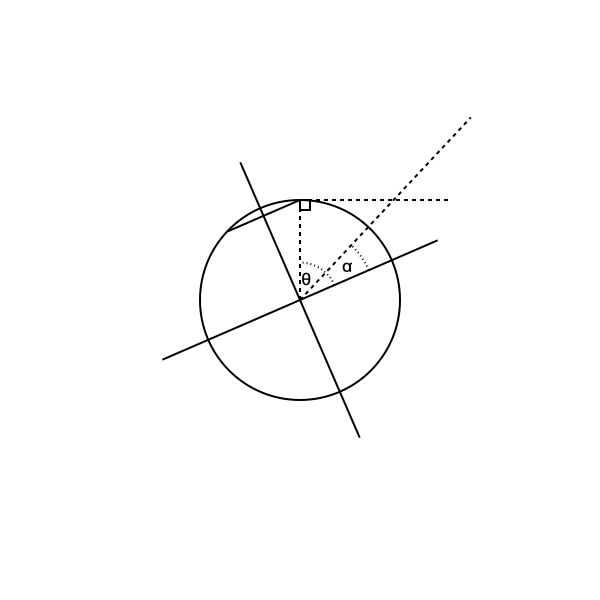
\includegraphics[width=0.5\textwidth]{EarthDiagram.png}
        	\centering
    		\caption{Cross-sectional Diagram of Earth (made diagram with Julia)}
    		\label{fig:Earth}
    	\end{figure}

	The variable \(\theta\) represents the angle formed between the equator and the line connecting the center of the Earth to the Arctic circle where the observer is standing. This is given as \(\theta=66.56 ^\circ \).\\
	
	
	The variable \(\alpha\) represents the angle formed between the equator and the Sun's declination. The Sun's declination can be divined by understanding that (a) because it is the Summer Solstice, the Sun is at it's maximum declination and (b) the latitude of the Tropic of Cancer corresponds directly with the maximum declination of the Sun. The Tropic of Cancer's latitude is given, therefore we know that \(\alpha=23.44 ^\circ \). \\
	
	
	Simple geometry yields:
	\[
		\begin{split}
			\chi = 90^\circ - (\theta - \alpha) = 90^\circ - (65.56^\circ - 23.44^\circ) = 46.88^\circ
		\end{split}
	\]
	
	By the Alternate Interior Angle Theorem, we can conclude that the altitude angle is equal to \(\chi=46.88 ^\circ \) \\

\end{homeworkProblem}

\pagebreak

\begin{homeworkProblem}
 	(a) Make a log-log plot of the orbit size (y-axis) versus the orbit period (x-axis) for the planets in the Solar System. You can look up periods (P: the time to complete one orbit, \underline{please use Earth Years}) and sizes (a: \enquote{semi-major axis} or average orbit radius for planets, \underline{please use \enquote{Astronomical Units}} (A.U.) - the size of the Earth's orbit is 1.0 A.U.) in a textbook or in any reputable on-line source. (b) What is the slope of the log-log plot? (c) Use this slope to write an equation to describe the relationship between period and orbital size. (Marks 7)\\
 	
 	\textbf{Solution}
 	
 	N.B. All plots, tables, and computations made with Julia. The data were taken from the textbook. \\
 	
 	\textbf{Part a}\\

	\begin{figure}[!h]
		\centering
		\begin{tabular}{rrr}
				\hline\hline
				\textbf{Name} & \textbf{Sidereal Period} & \textbf{Semimajor Axis} \\
				\texttt{} & \texttt{y} & \texttt{AU} \\\hline
				Mercury & 0.24 & 0.39 \\
				Venus & 0.6 & 0.72 \\
				Earth & 1.0 & 1.0 \\
				Mars & 1.88 & 1.52 \\
				Jupiter & 11.86 & 5.2 \\
				Saturn & 29.46 & 9.54 \\
				Uranus & 84.01 & 19.19 \\
				Neptune & 164.82 & 30.06 \\\hline\hline
			\end{tabular}
       	\caption{Table of orbital data for the major planets of the Solar System (data taken from textbook)}
    		\label{fig:data}
    	\end{figure}
    	
    	\begin{figure}[!h]
    		\centering
	    	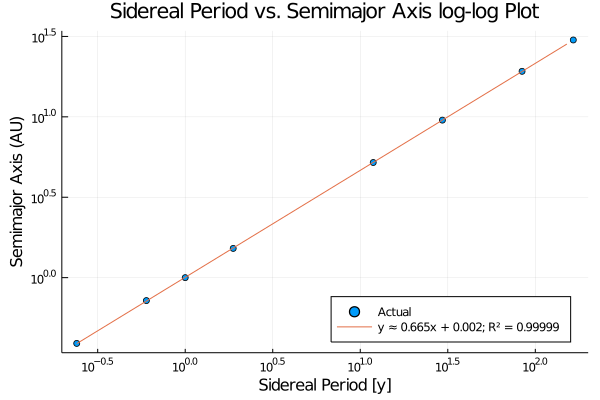
\includegraphics[width=0.75\linewidth]{SiderealPeriod_SemiMajorAxis_LogLogPlot.png}
	    	\caption{Log-log plot with best-fit line made with Julia}
    	\end{figure}
    	\pagebreak
    	
 	\textbf{Part b}

 	The slope of the best-fit line is approximately  \(0.665 \hspace{2pt}[AU/y]\). This was determined by computing the least squares regression on the data.\\
 	
 	
 	\textbf{Part c}
 	
 	The equation describing the best-fit line is: \(y \approx 0.665 x + 0.002 \hspace{2pt}[AU/y]\), where \(y\) represents semimajor axis distance in AU and \(x\) represents period in Earth Years. The R-Squared value, which quantifies the quality of the regression, is \(>0.99999\) indicating a very strong, positive correlation between these two parameters.\\
 	
 	Please see \href{https://github.com/zborffs/Astronomy.jl/tree/master/problems/ps1}{my github repo} for details on computations, data, plots, and figures for this problem set.
\end{homeworkProblem}

\pagebreak

\end{document}
